\documentclass{article}
\usepackage[T1]{fontenc}
\usepackage{lmodern}
\usepackage{graphicx}
\usepackage{amsmath,amssymb}
\usepackage[a4paper,margin=2cm]{geometry}
\usepackage[absolute,overlay]{textpos}
\setlength{\TPHorizModule}{1mm}
\setlength{\TPVertModule}{1mm}
\usepackage[indonesian]{babel}
\usepackage{hyperref}
\setlength{\emergencystretch}{2em}
% unit: Halaman 21

\begin{document}

% === Halaman 21 (llm) ===

\section*{Transformasi $ShiftRows()$}

\vspace{158.00mm}

\begin{itemize}
    \item Transformasi $ShiftRows()$ melakukan operasi permutasi dengan pergeseran secara $wrapping$ (siklik) pada 3 baris terakhir array state.
    \item Jumlah pergeseran bergantung pada nilai baris ($r$). Baris $r = 1$ digeser sejauh 1 $byte$, baris $r = 2$ sejauh 2 $byte$, dan baris $r = 3$ sejauh 3 $byte$. Baris $r = 0$ tidak digeser.
\end{itemize}

\vspace{10mm}

% deskripsi: Diagram ilustrasi transformasi ShiftRows pada array state, menunjukkan pergeseran siklik baris 1, 2, dan 3 dari matriks state ke state'.
% bbox normalisasi: [0.1080, 0.4140, 0.8880, 0.9460]
\begin{textblock*}{163.80mm}(22.68mm,122.96mm)
\noindent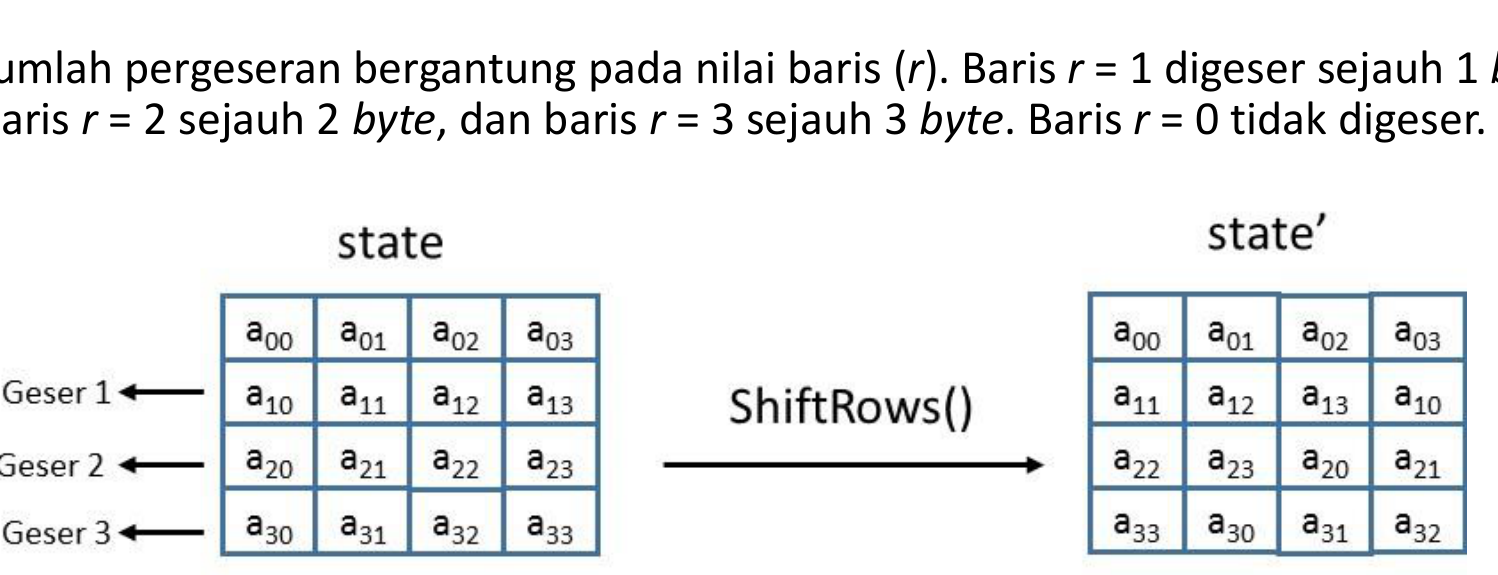
\includegraphics[width=163.80mm,height=158.00mm]{../../images/llm/page_021_img_01.png}%
\end{textblock*}

\end{document}
